\chapter{Design}

Til at styre de Bipolære stepper motorer anvendes der et print designet omkring chippen L298, der er en dual full-bridge driver.

På blok diagrammet for L298 der kan ses på figur \ref{blok298}, ses det at chippen indeholde mulighed for at lave et strøm feedback loop tilbage til PSoC 5 Chippen hvor man ved hjælp af en comparator og en DAC kan sikre sig mod for store strømme i stepper motoren. 

Derudover kan man se hvordan brugen af AND-Gates kan medføre en besparelse i antallet af pins der er nødvendige for at drive en full-bridge.

\begin{figure}[H]
	\centering
	\caption{Blokdiagram for L298, kilde: datablad for L298}
	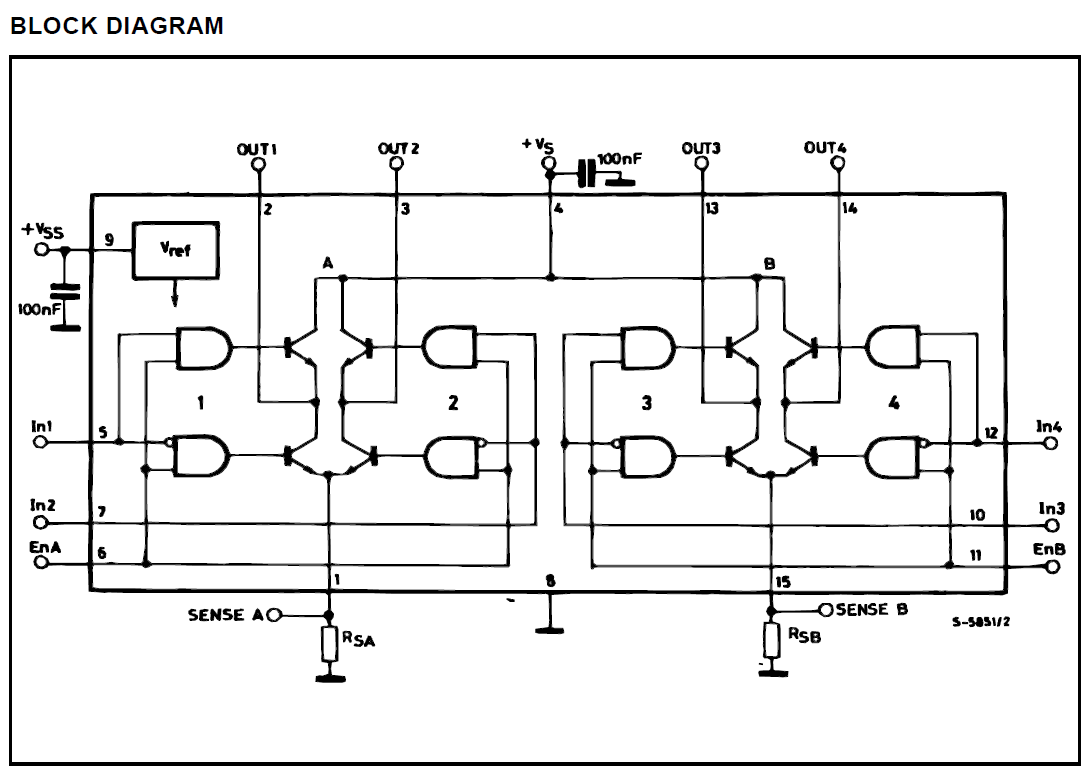
\includegraphics[scale=0.5]{billeder/blokdiagramL298}
	\label{blok298}
\end{figure}

Denne forsynes via 12V og 78L05 DC-DC 5V konverteren på boardet med 5V til de logiske enheder på chippen.

Derudover er der som anbefalet i databladet for 78L05 sat kondensatorer til at stabiliserer 5V forsyningen, samt på L298 ud fra anbefalinger i databladet.

\begin{figure}[H]
	\centering
	\caption{kredsløb til styring a bipolar steppermotor med L298 samt L297. Kilde: datablad L298.}
	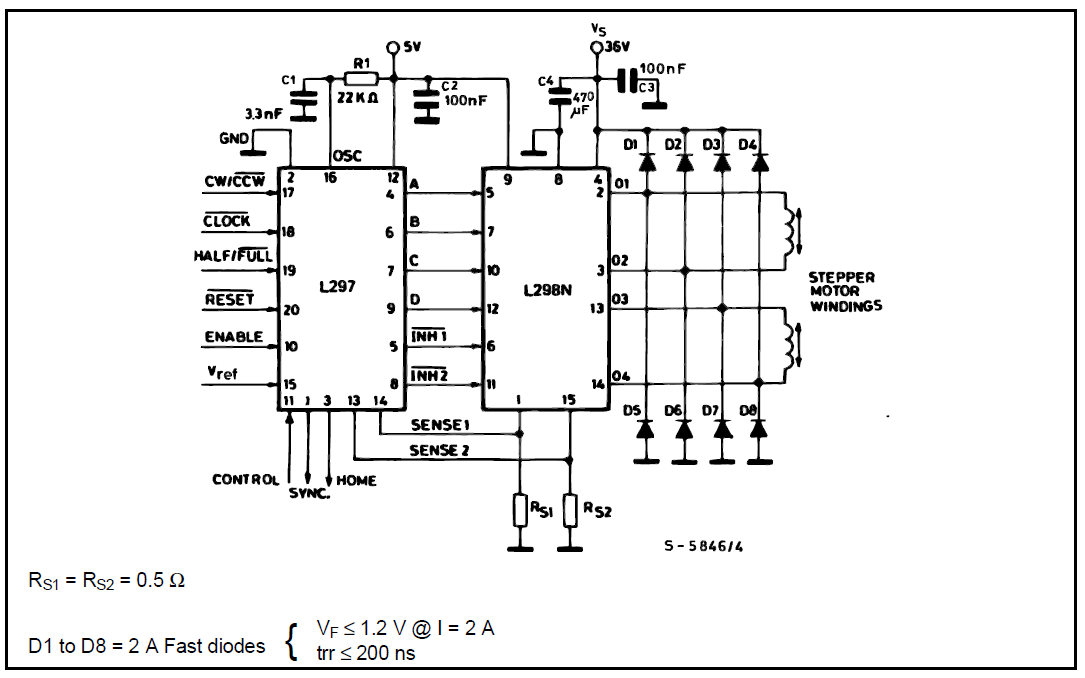
\includegraphics[scale=0.5]{billeder/kredsloebL297L298}
	\label{L298L297}
\end{figure}

Der er i designfasen taget udgangspunkt i kredsløbet der ses på Figur \ref{L298L297} , i vores kredsløb er L297 dog erstattet af en PSoC5LP og der er anvendt andre modstande til strømsfeedback delen, da vi ikke havde den samme type på lager på skolen.

Der i som RS1 og RS2 istedet anvendt en 0.1 ohm effektmodstand, da de små 1/4 watts modstande ikke ville kunne tåle de strømme der vil kunne løbe igennem motoren.

Dette giver os ud fra kirchoffs strømlov at strømmen gennem RS1 er den samme som strømmen gennem spolen på stepper motoren, derved kan vi ved hjælp af ohms lov finde frem til den spænding vi skal indstille vores DAC i PSoC5LP til, for at vi opnår den ønskede strøm i motoren.

Den generelle formel findes i ligning \ref{Currentfeedback-general} hvorfra en mere specifik udgave der kun vil passe på vores kredsløb kan findes på i ligning \ref{Currentfeedback-specific}

\begin{equation}
\label{Currentfeedback-general}
	\frac{I_{spole}}{R_{S1}}=V_{DAC}
\end{equation}

\begin{equation}
\label{Currentfeedback-specific}
\frac{I_{spole}}{0.1\Omega}=V_{DAC}
\end{equation}


	
